%\documentclass[main.tex]{subfiles}
%\begin{document}

\section{Radiation Field}

This chapter describes the radiation field inside the CHARM test area. With the many different facility configurations, there is a large variation in the particle and energies seen in the spectra at the various test locations. In order to understand what the field is like in the different test positions, the FLUKA Monte Carlo code has been used to simulate the radiation field. This starts with making an accurate model of the inside of the test area, correctly describing the beam and making reasonable assumptions about the running of the facility. \\

In order to make a thorough and complete analysis of the radiation field, it is important to decide what information is needed, and how it can be compared with real-life mixed radiation fields such as space or accelerator facilities. This step requires the formation of metrics and standards, in order to make accurate comparisons and consider the strength of the match. From there, tables of data can be produced for each position and each configuration, stating the matches for various comparisons. \\

A list of useful units is included in the appendix, table \ref{tab:useful_quantities}. \\

\subsection{Quantifying the Radiation Field}

There are many quantities which are useful to know during radiation tests, and these vary depending on the kind of test a user would like to make. It ranges from the simplest total ionising dose (TID) tests, where only the dose at the location as a function of time is needed, to very specific quantities such as 1MeV equivalent neutron fluence which is useful in studies of displacement damage in electronics. \\

The radiation environment inside the CHARM area is described as a 'mixed' field. This means that the radiation within the test area comes in many types, such as protons, neutrons, pions, etc, and of a wide range of energies. These originate from the beam interacting with the target. This is contrary to a gamma facility for example, where the field is only 1 type of radiation. In fact many radiation environments can be described as a mixed-field, such as in the upper atmosphere where one finds not only protons but also neutrons and muons, thus the types of radiation are 'mixed'. \\

At CHARM one can find an entire range of particles from the beam interaction with the target. At the test location one typically sees a number of hadrons (including protons, neutrons, pions and kaons), leptons (electrons, positions and muons) and photons (x-ray and gamma). These range in energy from near primary beam protons and neutrons at 24 GeV, to thermal neutrons from the test area wall scattering at \textless 1 eV. \\

\subsection{Metrics}

In order to compare the mixed-radiation field at CHARM with other fields, a metric needs to be defined in order to be able to describe and then compare radiation fields. This should give a clear and simple way to cross-compare, and should also show the strength of the fit. This could be either a single value, or a number of different tests that overall show the quality of the fit for that environment. \\

There are potentially many ways to compare different mixed radiation fields. There are fluences of various different particles of which have a variety of types and energies, all which have varying impacts on the operation of electronics and systems containing electronic components. To narrow the search down, one key factor that is important for SEEs is particle energy, and how it transfers the energy to sensitive part of the device. A measure of this is the 'linear energy transfer' (LET), and usually there is a minimum LET required to induce SEEs (depending on the specific device or system). To further narrow the search, typically the only kind of particles that can cause reactions which produce particles with LETs large enough to cause SEEs are hadrons. Therefore the area of interest for SEEs in electronics is usually hadrons with a high enough energy (LET) to cause the problems we are trying to avoid \cite{rad_effects_handbook}. \\

% Explain HEH, HEHeq, r, n_thrm

Before introducing the metrics describing the radiation field, it is important to define some quantities used in the metrics. The first is called the 'high-energy' hadrons (HEH), which corresponds to all hadrons above an energy of 20 MeV. This particular energy is chosen since this energy corresponds to a rough minimum required to cause SEEs. There is a second similar value called the high-energy hadron equivalent (HEHeq). The difference lays in the way the fluence of hadrons below 20 MeV is calculated. In this case, instead of a minimum threshold, a Weibull function is used to model the response of a typical SRAM used for SEU detection (in the Radmon system for example). This response is then assumed to be more accurate than the former method for defining the HEH fluence. \\ 

Two further values of interest that can be helpful when defining the metrics are the 'r factor' and the thermal neutron equivalent fluence. The r factor (or risk factor) is the ratio between the fluence of thermal neutrons to HEH. Since thermal neutrons can cause problems due to the ionisation of products of nuclear capture reactions within the electronics, it is important to define their contribution from the overall hadron fluence \cite{Baumann2001211}. The sensitivity of electronics to thermal neutrons is not always well tested for, and thus the risk of placing electronics in a field that contains thermal neutrons is very useful to know. The r factor can be calculated using the Radmon system by making multiple measurements at a specific location with different detector biases \cite{Kramer:1399765}. \\

The thermal equivalent fluence is calculated by taking the thermal neutron fluence and folding with a 1/v weighting to replicate the capture cross-section of neutrons in boron 10. This is relevant to studies of SEEs in electronics since boron 10 was previously found in a number of electronic components due to certain manufacturing processes and the products from the nuclear reactions have a high enough LET to induce SEEs \cite{Baumann2001211}.\\

The first metric that could be used are the 'hardness factors', which quantify range of energies of high energy hadrons in a radiation environment. To calculate these factors, one takes the simulated high energy hadron spectrum and makes a reverse integral, normalised to 1 at 20MeV. From this, the values at 50\% and 10\% (H50 and H10) are taken, which correspond to the proportion of the HEH fluence above this energy. \\

A second way to make a comparison between data-sets and real measurements could be to use the fission cross-section in Tungsten for devices where the material is used. The importance of Tungsten is from the fragments caused during fission reactions. These fragments have a large LET and thus deposit large amounts of charge, which maybe be close to the active volume of the electronics \cite{1589248}. \\

The method involves taking the simulated proton-induced Tungsten fission cross-section and folding this with the simulated normalised HEH fluence. The integral of the folded spectrum will give the probability of a fission event in Tungsten for this HEH spectrum. For a comparison with a real value, one can divide this by the 230 MeV proton induced fission cross-section in Tungsten. Then, if one tests a device in a 230 MeV proton beam, the ratio will give an indication of how the number of events could scale in the simulated HEH spectrum. An example of this method is shown in figure \ref{fig:w_factor_example}, which gives a ratio of 1.322 between the expected cross-section in the mixed-field at this location and configuration and the cross-section at 230 MeV. \\

\begin{figure}[!ht]
	\centering
	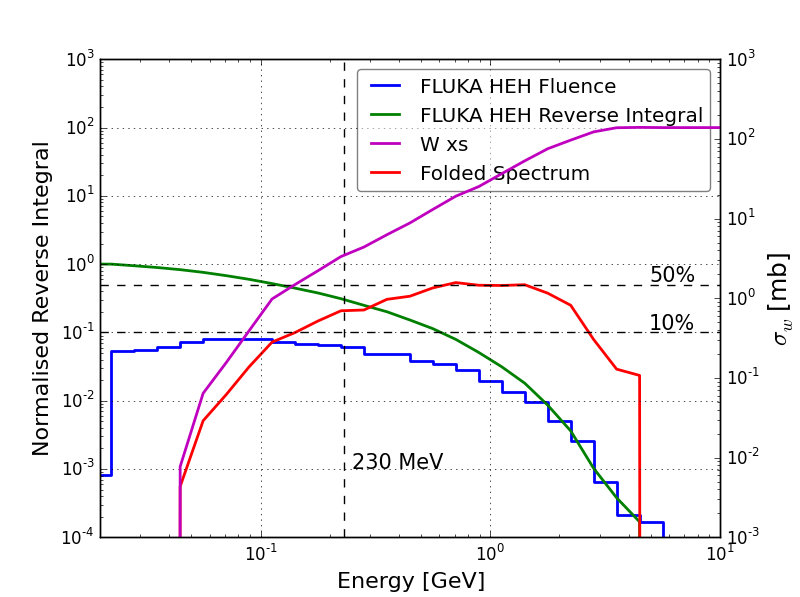
\includegraphics[width=0.7\textwidth]{./images/w_folded_spectrum3}
	\caption{A plot of the HEH fluence for a specific test position, folded with the Tungsten fission-fragment cross-section, giving a 'response' for a detector in which the SEU sensitivity is dominated by the Tungsten inside the device. A reference of 230 MeV is used to compare with results with those obtained during tests at PSI in Switzerland. Also plotted is the HEH reverse integral spectra, with the corresponding H10 and H50 factors.}
	\label{fig:w_factor_example}
\end{figure}

\clearpage
\subsection{Standards and Environments}

There are a number of different environments (natural or otherwise) which have been studied to calculate the radiation field. The different radiation types, energies and fluences are calculated  for each environment and tabulated, but to be able to compare them, some standards have to be created. As shown in the previous section, one way to compare different mixed-field radiation environments is to use the 'hardness-factor' which is related to the fluence of high-energy hadrons, and gives information about the energy and flux of hadrons. A collection of these values, including spectral information is shown in table \ref{tab:hardness_energies}. The data for the various LHC areas is given for nominal conditions (50fb$^{-1}$). \\

%For TID testing, there are a range or standard dose rates... (need table) ELDR..\\

%Description and reference to some different environments (spectra plots?) \\

\begin{table}[htbp]
\small
  \centering
    \begin{tabular}{l|p{1.8cm}|r|r|r|r|r|r|r|r}
    \textbf{Environment} & \textbf{HEH /cm$^{2}$/ y} & \multicolumn{4}{c|}{\textbf{Composition (\%)}} & \textbf{R} & 				\multicolumn{3}{c}{\textbf{Hardness Energy}} \\ \cline{3-6} \cline{8-10}  
    & & n & p & pi$^{+-}$ & n$_{int}$ & & H50 & H10 & H1 \\
    \hline
    \hline
    CERN - LHC UJ 				& 2.5E+09 & 99    & 1     & 0     & 32    & 2     & 0.08  & 0.18  & 0.36 \\
    CERN - LHC RR 				& 1.0E+09 & 71    & 13    & 16    & 25    & 10    & 0.18  & 0.69  & 2.8 \\
    CERN - LHC Tunnel 			& 6.0E+11 & 45    & 18    & 37    & 19    & 2.8   & 0.37  & 1.8   & 5.7 \\
    CERN - ATLAS Outer Tracker 	& 3.5E+09 & 67    & 5     & 28    & 25    & 1.1   & ?     & 0.46  & 0.71 \\
    CERN - ATLAS Inner Tracker 	& 1.0E+12 & 4     & 7     & 89    & 1     & 2     & 1.5   & 3.8   & 12 \\
    CERN - LINAC 4 				& 1.0E+10 & 99    & 1     & 0     & 86    & 1.5   & ?     & 0.07  & 0.1 \\
    CERN - PS 					& 1.0E+11 & 61    & 17    & 22    & 19    & 4.9   & ?     & 0.9   & 2.4 \\
    CERN - SPS 					& 1.0E+12 & 70    & 12    & 18    & 29    & 48.9  & ?     & 0.94  & 5.1 \\
    QARM - 350m (Geneva, CH) 	& 1.6E+05 & 93    & 7     & 0     & 21    & 0.12  & 0.08  & 0.34  & 1.3 \\
    QARM - 10km (Geneva, CH) 	& 1.7E+07 & 82    & 18    & 0     & 18    & 0.08  & ?     & 0.92  & 5 \\
    QARM - 20km (Geneva, CH) 	& 3.8E+07 & 68    & 32    & 0     & 14    & 0.06  & 0.5   & 2.9   & 13 \\
    CREME 96 - ISS (450km) 		& 7.3E+08 & -     & -     & -     & -     & -     & ?     & 0.25  & 0.53 \\
    CREME 96 - Proba II (800km) & 2.7E+09 & -     & -     & -     & -     & -     & 0.1   & 0.28  & 1.5 \\
    \end{tabular}%
  \caption{Table of hardness energies for various radiation environments \cite{radecs2014shortcourse}. The hardness factors for the spectra calculated with CREME96 used protons only. The 'n$_{int}$' component stands for the intermediate neutrons, which are those with an energy between 0.2 MeV and 20 MeV. The hardness energies are given in GeV.}
  \label{tab:hardness_energies}%
\end{table}%

% 1E9 HEH = approx 1 Gy. These are from the nominal conditions. Hi-Lumi factor 10? Starting 2024 (after LS3) \\

%Add a column of dose rates per year to compare \\

%Add the references to the LHC areas (for example, which UJ does this refer to?) \\





\newpage
\subsection{FLUKA Calculations}

The FLUKA Monte Carlo code \cite{FLUKA1} \cite{FLUKA2} was used to perform the radiation field calculations for the CHARM test area. For this, a geometry was built specifically for CHARM test area. This geometry includes all the main features of the test area; i.e. the target table with the 3 different targets, the movable shielding, the different materials in the surrounding shielding walls, the exact test positions etc. An effort was made to make the geometry as accurate as possible with respect to the technical drawings and double-checked with measurements made in the facility, in order to reduce the errors with respect to positioning. Care needed to be taken as the variations in the radiation field with respect to position (gradients) can be high for areas close to the beam and down-stream of the target. \\

\subsubsection{FLUKA Geometry}

An accurate model was made specifically using FLUKA for the CHARM area. Details and dimensions were taken from a combination of CATIA 3D drawings, and then finally measurements once the facility had been constructed. It was decided to focus on the details around the test area, therefore the geometry as seen in FLUKA includes only the first layer of shielding. This will optimise the time used during the calculations by not tracking the particles in area that are not of interest. \\

The co-ordinate system for the FLUKA geometry was defined with the z axis parallel with the beam, y axis for the height, and the x axis adjacent to the beam. This will then be used in the rest of the document when describing the radiation field. These along with the test positions can be seen in figure \ref{fig:fluka_test_positions}.\\


\begin{figure}[!ht]
	\centering
	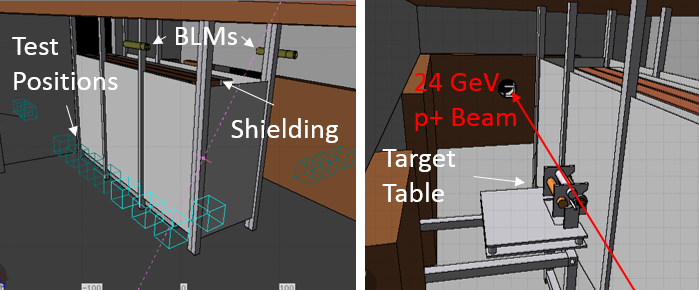
\includegraphics[width=0.9\textwidth]{./images/fluka_charm_shielding_ann2}
	\caption{A screen-shot of a cut of the FLUKA geometry, showing the shielding and test position scorings (in blue). The BLMs are also visible at the top of the shielding.}
	\label{fig:fluka_screenshot}
\end{figure}

\begin{figure}[!ht]
\centering
\begin{subfigure}{.5\textwidth}
  \centering
  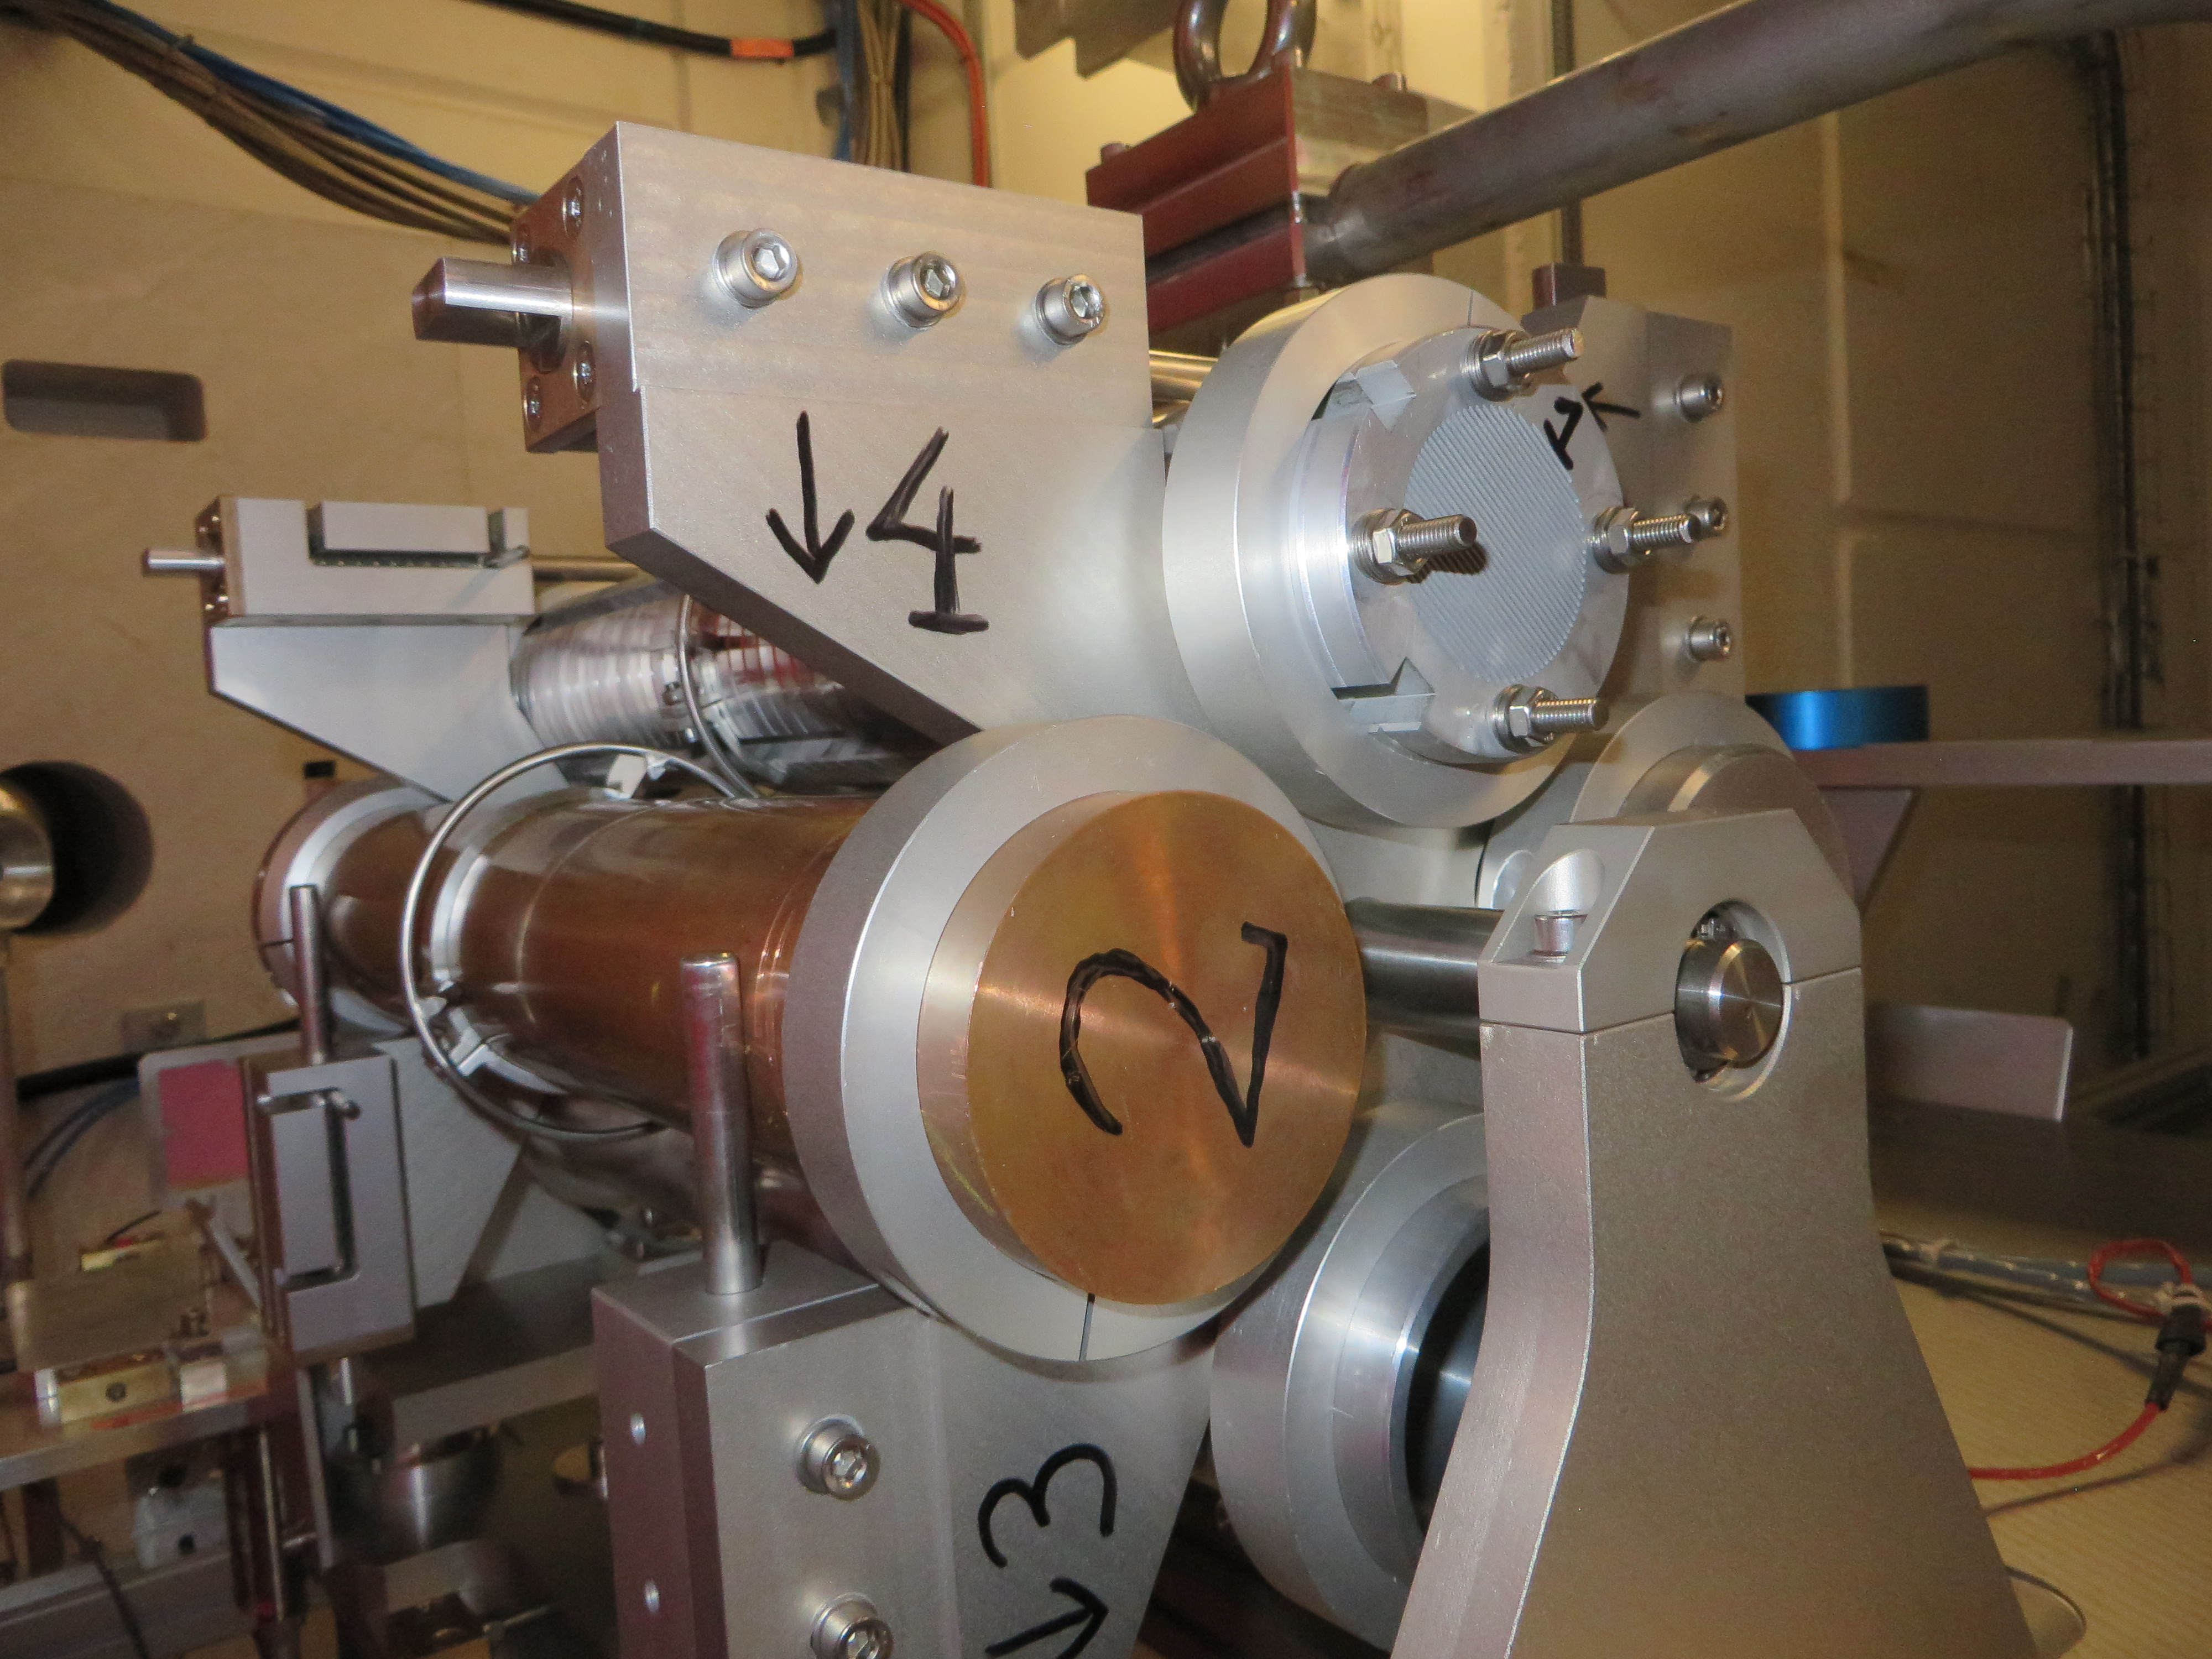
\includegraphics[width=0.9\linewidth]{./images/IMG_1149}
  \caption{A photo of the target table.}
  \label{fig:fluka_target_photo}
\end{subfigure}%
\begin{subfigure}{.5\textwidth}
  \centering
  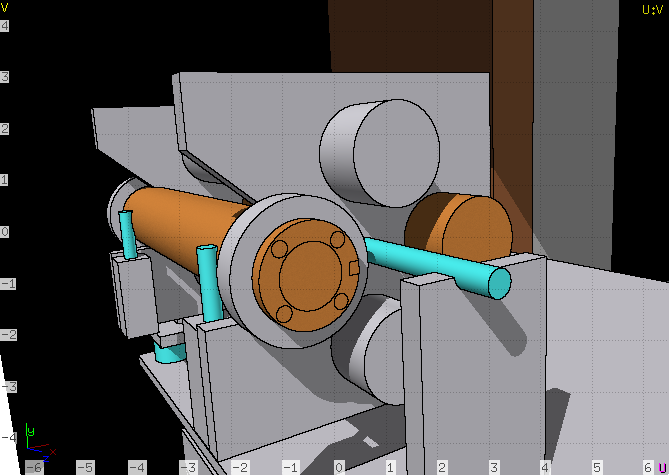
\includegraphics[width=0.9\linewidth]{./images/target_photo_perspective}
  \caption{A screen-shot from the FLUKA geometry}
  \label{fig:fluka_target_geometry}
\end{subfigure}
\caption{A comparison of the real target station and the simplified target station implemented in the FLUKA geometry.}
\label{fig:fluka_target_comparison}
\end{figure}

\subsubsection{FLUKA Physics Configuration}

In FLUKA it is possible to configure the transport of certain particles and likelihood of interactions by changing specific parameters or adding special cards into the input file. The motivation for these is to 'tune' the simulation so that a satisfactory level of accuracy is met, which is usually to do with the statistical uncertainty calculated by the various scoring implemented in the input file, without causing an adverse effect on CPU time. An example of this is the transport threshold for electrons and positrons which can be set to any energy desired. On one hand it's possible to raise the thresholds (or even stop the transport completely) to a level that could even cause non-physical artefacts in the scoring for dose for example, which would reduce the CPU vastly. On the other extreme it's possible to reduce the energy to a level where non-physical effects are very low, but the CPU time per primary particle in the simulation becomes a limiting factor when trying to gain an acceptable level of accuracy in terms of statistics. \\

It was decided to use the NEWDEFA PHYSICS card in the 'defaults' for the CHARM test area calculations with the transport of electrons enabled. This has a 1MeV transport threshold for delta-rays (electrons), which gives a reasonable level of accuracy without greatly impacting the CPU time of the simulation. No biasing was set for the regions inside the test area and no other thresholds were modified. \\

\subsubsection{Scoring}

There are a number of estimators built into FLUKA for calculated various quantities, such as charge particle fluence, dose in air etc. Deciding which estimators to use and how to normalise the data depends on the purpose of the simulation. For the CHARM facility, the focus is on testing of electronics, for which there are a number of appropriate estimators for this purpose. One example is scoring 'high-energy hadrons' i.e. the total flux of hadrons above 20 MeV (deemed the cut-off energy for SEE's in electronics). The selection used for the CHARM FLUKA studies is listed below.

\begin{table}[htbp]
  \sisetup{tight-spacing=true}
  \centering
    \begin{tabular}{l|p{9cm}}
	Estimator & Physical Meaning \\
	\hline
	\hline
	DOSE		& The energy deposited per unit mass \\
	HADGT20M	& Fluence of Hadrons with energy above 20 MeV \\
	SI1MEVNE	& Fluence of 1 MeV (Si) equivalent neutrons \\
	NEUTRON		& Fluence of neutrons \\
	HEHAD-EQ	& Fluence of Hadrons with energy above 20 MeV including intermediate neutrons \\
	THNEU-EQ	& Fluence of thermal-equivalent neutrons \\
    \end{tabular}
	\caption{A table of the estimators used for the CHARM FLUKA calculations. A detailed list can be found in the appendix in table X. More details available in the FLUKA manual.}
	\label{tab:fluka_estimators}
\end{table}